\documentclass[12pt]{article}
\usepackage[utf8]{inputenc} 
\usepackage[english, russian]{babel} 
\usepackage{amsmath,amsfonts,amssymb,euscript,graphicx,wrapfig,multirow}
\usepackage{dsfont}
\usepackage{amsthm}
\textheight=240mm \textwidth=170mm
\hoffset=-17mm % сдвиг влево
\voffset=-17mm % сдвиг вверх

\usepackage{hyperref}

\theoremstyle{theorem}
\newtheorem{theorem}{Теорема}
\theoremstyle{dfn}
\newtheorem{dfn}{Определение}
\theoremstyle{remark}
\newtheorem{remark}{Замечание}

\begin{document}

\selectlanguage{russian}

\noindent УДК

\begin{center}
\textbf{О некоторых оценках диаметра целоудалённых множеств точек более высоких размерностей} \\[3mm]
\textbf{Р.~Е.~Зволинский, Е.~А.~Момот} \\[2mm]
\emph{ВГУ}
\end{center}

\section{Введение}

\begin{dfn}\label{dfn1}
	Плоским целоудалённым множеством точек (ЦМ) называют такое 
	множество $\mathcal{P}$ не лежащих на одной прямой точек на 
	плоскости $\mathbb{R}^{2}$, таких, что для любой пары 
	точек $P_{1}, P_{2} \in \mathcal{P}$ 
	расстояние $|P_{1}P_{2}|$ между точками $P_{1}$ и $P_{2}$ есть целое число.
\end{dfn}

Определение \ref{dfn1} можно обобщить для общего случая:

\begin{dfn}
	Целоудалённым множеством $\mathcal{P}$ называют множество из $n$ точек в
	$m$-мерном Евклидовом пространстве $\mathbb{R}^{m}$ с
	попарными  целочисленными  расстояниями между точками данного множества.
\end{dfn}

Как можно охарактеризовать такое целоудалённое множество?
Во-первых, мы можем посмотреть на его размерность,
тогда у нас получится посчитать число точек данного множества, которое всегда конечно [1, 2], далее будем называть это число \textit{мощностью};
наконец, мы можем естественно определить диаметр такого конечного набора точек.

\begin{dfn}
	Диаметр ЦМ $\mathcal{P}$ опеделяется как
	\begin{equation}
		\operatorname{diam(\mathcal{P})} = \underset{P_{1}, P_{2} \in
		\mathcal{P}}{\max} |P_{1}P_{2}|
	\end{equation}
\end{dfn}

У каждого ЦМ также есть характеристика
[3, 4].

\begin{dfn}
	Функция $d(m, n)$ есть минимальный возможный диаметр ЦМ $\mathcal{P}$ из $n$ 
	точек в $m$-мерном Евклиловом пространстве $\mathbb{R}^{m}$.
\end{dfn}


Спискок известных оценок функции $d(m, n)$
читатель может найти в [5, Theorem 1] или в [6].
Мы обсудим следующие оценки, представленные в [5]:
\begin{align}
	&d(m, 2m + 1) \leq 8\\
	&d(m, 2m + 2) \leq 13 \hypertarget{d2}\\
	&d(m, 3m) \leq 109
\end{align}
и следующую теорему [5, Theorem 2.1].

\begin{theorem}
	Пусть $\mathcal{P}$ это плоское целоудалённое множество точек, 
	где $n - 2$ точки  расположены на прямой $l_{1}$, а две точки 
	$P_{1}$ и  $P_{2}$ на параллельной ей прямой $l_{2}$ с расстоянием 
	$r$ между $l_{1}$ и $l_{2}$. Если существуют такие положительные целые числа 
	$v$, $w$, удовлетворяющие условиям $f^{2} + v^{2}
	= w^{2}$ и $v < 2r$, где $|P_{1}P_{2}| = f$,
	то

	\begin{equation}\label{formula1}
		d(m, n - 2 + 2(m - 2)) \leq \max(w, \operatorname{diam(\mathcal{P})})
	\end{equation}

\end{theorem}

В данной статье мы представим некоторые оценки функции $d(m,n)$, основанные на плоских ЦМ определённых типов.

\section{ЦМ, расположенные на двух прямых}

\begin{dfn}
    Плоские целоудалённые множества точек, расположенных на двух параллельных прямых, будем называть рельсовыми системами.
\end{dfn}

Среди рельсовых систем наиболее распространены ЦМ с двумя точками на одной прямой и остальными на другой.


\begin{dfn}
    Плоские целоудалённые множества точек, расположенных на двух прямых, 
    не являющихся ни параллельными, ни перпендикулярными, будем называть системами
    типа ножницы.
\end{dfn}

Существует важный подкласс наборов ножниц.

\begin{dfn}
    Системы типа ножницы с осью симметрии, 
    являющейся биссектрисой угла между прямыми, назовём пирамидальными.
\end{dfn}

\section{Оценки, основанные на рельсовых системах}

Пусть $i = \overline{1, k}$ обозначает перечисление всех $i$
от $1$ до $k$.
Теорему [5, Theorem 2.1] можно обобщить для общего случая
следующим образом:

\begin{theorem}
	Пусть $\mathcal{P}$ это плоское целоудалённое множество точек, где 
	$n - k$ точек расположены на прямой $l_1$, а $k$ точек $P_1$, $P_2$, $\ldots$,
	$P_k$ на параллельной ей прямой $l_2$ с расстоянием $r$ между $l_1$ и $l_2$. 
	Если существуют такие положительные целые числа $v$, $w_{ij}$, удовлетворяющие
	условиям $f_{ij}^{2} + v^{2} = w_{ij}^{2}$ и $v < 2r$, где 
	$i = \overline{1, k - 1}$, $j = \overline{i + 1, k}$, $|P_{i}P_{j}| = f_{ij}$,
	то

	\begin{equation}
		d(m, n - k + k(m - k)) \leq \max(w_{1k}, \operatorname{diam(\mathcal{P})})
	\end{equation}
	
\end{theorem}

Ниже мы приводим оценки функции $d(m, n)$ для $n = 2m + k$, $3 \leq k \leq 24$, а также для $n = 4m$, основанные на рельсовых ЦМ (подробное описание данных ЦМ и конструкций для построения оценок можно найти в [7]).
\begin{align*}
&(d(m, 2m + k))_{k = 3, \ldots, 24} \leq 158,\, 158,\, 252,\, 297,\, 1073,\, 1273,\, 1888,\, 2189,\, 3224,\, 3696,\, 5141,\, 6586,\, \\
&11692,\, 12296,\, 16027,\, 19758,\, 32054,\, 39516,\, 254364,\, 276612,\, 338169,\, 399726
\end{align*}

Ричард Гай в своей работе [8, D 20] приводит ЦМ из $8$ точек, расположенных на двух параллельных прямых. На основании данной ЦМ там удалось получить оценку
\begin{equation}\label{result1}
d(m, 4m) \leq 409
\end{equation}

Также с помощью мощностей ЭВМ нам удалось получить рельсовую ЦМ мощности 40 (на данный момент это наибольшая по мощности рельсовая ЦМ, которую нам удалось найти).
Ниже приведен иллюстрированный пример данной ЦМ.

Для облегчения восприятия применяется запись вида 
[9, 10, 6]:
$\sqrt{p}/q * \{ (x_1,y_1), \ldots,$ $ (x_n, y_n)  \}$,
означающая, что каждую абсциссу нужно умножить на $1/q$,
а каждую ординату~--- умножить на $\sqrt{p}/q$, т.е.
$$
	\sqrt{p}/q * \{ (x_1,y_1), ..., (x_n, y_n)  \}
	=
	\left\{ \left(\frac{x_1}{q},\frac{y_1\sqrt{p}}{q}\right), ..., \left(\frac{x_n}{q},   \frac{y_n\sqrt{p}}{q}\right)  \right\}.
$$

\begin{figure}[h!]
	\begin{center}
	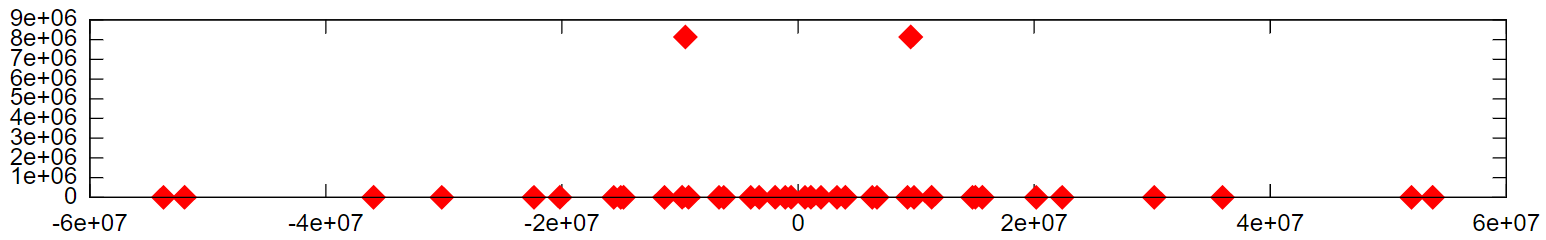
\includegraphics[width=1.1\linewidth]{picture_40.png}
	\parbox{1\linewidth}{\caption{ЦМ мощности 40, диаметр 107526848}
	\label{picture_40.png}}
	\end{center}
\end{figure}

\begin{itemize}
\setlength{\itemsep}{-1mm}

\item
$\mathcal{P}=\sqrt{154}/{1} * \{ (\pm 53763424, 60),
(\pm 51964380 , 0),
(\pm 35959560 , 0),
(\pm 30175080 , 0),
(\pm 22378720 , 0),
$

$
(\pm 20180160 , 0),
(\pm 15613780 , 0),
(\pm 15025920 , 0),
(\pm 14779380 , 0),
(\pm 11313120 , 0),
(\pm 9817080 , 0),
$

$
(\pm 9544080 , 655200),
(\pm 9271080 , 0),
(\pm 6693960 , 0),
(\pm 6289920 , 0),
(\pm 4006275 , 0),
(\pm 3290560 , 0),
$

$
(\pm 1938720 , 0),
(\pm 1092000 , 0),
(\pm 583648 , 0)\}
$
(Figure~\ref{picture_40.png}).

$f = 19088160$, $v = 8738$, $w = 19088162$, $\operatorname{diam(\mathcal{P})}
= 107526848$,

что даёт оценку $d(m, 2m + 34) \leq 107526848$.

\end{itemize}


\section{Оценки, основанные на пирамидальных системах}

\begin{theorem}
Пусть $\mathcal{P}$ это плоское целоудалённое множество точек, где
$k$ точек расположены на прямой $l_{1}$ и $k$ точек на прямой $l_{2}$.
Кроме того, эти точки симметричны относительно одной из биссектрис углов пересечения 
прямых $l_{1}$ и $l_{2}$, тогда

\begin{equation}\label{formula2}
d(m, (k - \alpha)m + \alpha) \leq \operatorname{diam(\mathcal{P})},
\end{equation}

где
\begin{equation*}
\alpha =
\begin{cases}
1, \text{если точка пересечения} \in \mathcal{P}, \\
0, \text{если точка пересечения} \notin \mathcal{P}.
\end{cases}
\end{equation*}

\end{theorem}

\begin{remark}
Углы могут быть острыми или тупыми. В [7] описано, почему угол пересечения прямых $l_{1}$ и $l_{2}$ не может быть равен ${\pi}/2$.
\end{remark}

Ниже мы приводим оценки функции $d(m, n)$ для $n = 3m + 1$ и $n = 4m + 1$, основанные на пирамидальных ЦМ (подробное описание данных ЦМ и конструкций для построения оценок можно найти в [7]).

\begin{align}
&d(m, 3m + 1) \leq 56 \label{result2} \\
&d(m, 4m + 1) \leq 1260 \label{result3}
\end{align}

Получившаяся оценка для функции $d(m, 3m + 1)$ улучшает оценку для $d(m, 3m)$, представленную в [3].

\section{Заключительное замечание}

Все данные ЦМ были получены путём сочетания копьютерного поиска и интуиции авторов;
таким образом, дальнейший поиск может привести к лучшим оценкам, использующим ту же
конструкцию.

До сих нет общей конструкции для рельсов или ножниц заданной мощности.

Для рельсовых ЦМ мы можем предположить, что существует множество произвольной мощности с $2$ точками на одной линии, а все остальные на другой; с другой стороны,
мы до сих пор не нашли ни одной рельсовой ЦМ с $4$ и $5$ точками на отделившихся прямых.

На сегодняшний день мы нашли пирамидальную ЦМ мощности не более $9$.

Исходный код можно получить по адресу https://gitlab.com/Nickkolok/ips-algo

\bigskip\centerline{\bf Литература}

1.	\emph{ Anning N.~H., Erd{\"o}s P.} Integral distances // Bulletin of the American Mathematical Society. -- 1945. -- Vol. 51, no. 8. -- Pp. 598-600. -- DOI: 10.1090/S0002-9904-1945-08407-9.

2.	\emph{ Erd{\"o}s P.} Integral distances // Bulletin of the American Mathematical Society. -- 1945. -- Vol. 51, no. 12. -- P. 996. -- DOI: 10.1090/S0002-9904-1945-08490-0.

3.  \emph{ Kemnitz A.} Punktmengen mit ganzzahligen Abst{\"a}nden. -- 1988.

4.  \emph{ Kurz S.} On the characteristic of integral point sets in $\mathbb{E}^m$ // Australasian Journal of Combinatorics. -- 2006. -- Vol.~36. -- Pp. 241-248. --
arXiv: math/0511704.

5.  \emph{ Kurz S., Laue R.} Bounds for the minimum diameter of integral point sets
// Australasian Journal of Combinatorics. -- 2007. -- Vol.~39. -- Pp. 233-240. --
arXiv: 0804.1296.

6.  \emph{ Авдеев Н.~Н., Семёнов Е.~М.} Множества точек с целочисленными расстояниями на плоскости и в евклидовом пространстве // Математический форум 
(Итоги науки. Юг России). -- 2018. -- Pp. 217-236.

7.  \emph{ Avdeev N.~N., Zvolinsky R.~E., Momot E.~A.} On particular diameter bounds
for integral point sets in higher dimensions. -- 2019. -- arXiv: 1909.10386v1

8.  \emph{ Guy R.} Unsolved problems in number theory. Vol. 1. -- Springer Science \& Business Media, 2013. -- DOI: 10.1007/978-1-4757-1738-9.

9.  \emph{ Авдеев Н.~Н.} On integral point sets in special position // Некоторые вопросы анализа, алгебры, геометрии и математического образования: материалы международной молодежной научной школы <<Актуальные направления математического анализа и смежные вопросы>>. -- 2018. -- Vol.~8. -- Pp. 5-6.

10.  \emph{ Авдеев Н.~Н.} Об отыскании целоудалённых множеств специального вида
// Актуальные проблемы прикладной математики, информатики и механики -- 
сборник трудов Международной научной конференции. -- Научно-исследовательские публикации, 2018. -- Pp. 492-498.

\end{document}



